\documentclass[12pt,a4paper,titlepage]{report}
\usepackage[utf8]{inputenc}
\usepackage[T1]{fontenc}
\usepackage[english,serbian]{babel}
\usepackage{amsmath}
\usepackage{amsfonts}
\usepackage{amssymb}
\usepackage[backend=biber]{biblatex}
\usepackage[babel]{csquotes} % Biblatex complains when this is not used.
\usepackage[unicode]{hyperref} % Links.
\usepackage{microtype} % Greatly improves word spacing in paragraphs.
\usepackage{parskip} % Nicer parskip, with no parindent.
\usepackage{graphicx} % Pretty images.
\usepackage{tabularx} % Tables.
\usepackage{tikz} % Diagrams.
\usetikzlibrary{shapes.multipart}
\usetikzlibrary{positioning}
\tikzset{entity/.style={
    draw=black,
    fill=yellow!16,
    rectangle split,
    rectangle split parts = 2,
    rectangle split part align={center,left}
}}
\usetikzlibrary{arrows.meta}
\usepackage{listings} % Code listings.
\lstset{
    language=SQL,
    captionpos=b,
    basicstyle=\ttfamily\scriptsize,
    numberstyle=\tiny,
    numbers=none,
    aboveskip=\bigskipamount,
    belowskip=\bigskipamount,
    backgroundcolor=\color{gray!10},
    frame=shadowbox,
    tabsize=2,
    rulecolor=\color{black!30},
    escapechar={\@},
    showspaces=false,
    showstringspaces=false,
    breaklines=true,
    breakatwhitespace=true,
    framextopmargin=2pt,
    framexbottommargin=2pt,
    extendedchars=false,
    inputencoding=utf8
}
\usepackage[titletoc]{appendix}
%\usepackage{float}
\graphicspath{{images/}}
%\setlength{\parskip}{0.5em}

\addbibresource{literatura.bib}
\author{Dimitrije Radojević \\ br. ind. 09/0112 \\ Elektrotehnički fakultet, Univerzitet u Beogradu}
\title{Diplomski rad}
\date{20. septembar 2016.}
\begin{document}
\maketitle
\tableofcontents
\chapter{Uvod}
Proba
\chapter{Zahtevi za realizacijom sistema}\label{zahtevi}
\section{Korisnički zahtevi}
Korisnički zahtevi se mogu podeliti u dve grupe. To su:
\begin{enumerate}
\item Zahtevi platforme generalne namene za polaganje, ocenjivanje i administraciju testova
\item Zahtevi sistema za parsiranje, transformisanje i prikazivanje logičkih izraza
\end{enumerate}
\subsection{Prva grupa zahteva}
Prva grupa zahteva se odnosi na samu platformu za polaganje testova. \subsubsection{Logovanje i registracija}
Kako je sistem namenjen za upotrebu od strane studenata i administratora, neophodno je implementirati logovanje postojećih korisnika na sistem i registraciju novih korisnika. Pri tom je bitno razlikovati login standardnih korisnika i administratora. Osim toga što ove dve role koriste sistem na različit način, administrator ima neke privilegije koje nisu dostupne običnom korisniku - na primer, pregledanje rezultata testova. O ovome se mora voditi računa, tako da se onemogući pristup resursima za koje su potrebne administratorske privilegije.

Logovanje treba da se vrši preko studentskog email naloga i lozinke. Novi korisnici se registruju tako što unesu email adresu, na koju se potom šalje nasumično generisana lozinka. Lozinke se od klijenta ka serveru treba da se šalju u heširanom obliku, a u istom obliku treba da se pohranjuju u bazi podataka. Administratoski nalozi se automatski ubacuju u bazu prilikom konfiguracije sistema.

Nakon što se korisnik uloguje, preko kolačića u pregledaču treba da se pamti korisnička sesija, i time izbegava ponovno, nepotrebno logovanje na sistem nakon napuštanja stranice. Sesije treba da ima određeno vreme validnosti, nakon kojeg je neophodno da se korisnik ponovo uloguje.

Korisnik treba da ima izbor da se izloguje kada poželi, i time invalidira korisničku sesiju.

\subsubsection{Pregled testova}
Nakon uspešnog logovanja, korisnik treba da vidi spisak svih testova koje trenutno može da polaže, testova čije je polaganje u toku, i testova koji su završeni, i to grupisanih po oblastima.

Testovi koji su završeni trebaju biti onemogućeni, tj. korisniku ne sme biti dozvoljeno da više puta polaže isti test. Za ovakve testove treba naznačiti i datum polaganja i uspešnost, tj. broj pitanja na koje je student tačno odgovorio u odnosu na ukupan broj pitanja na testu.

Za testove koji su u toku, tj. čije je polaganje korisnik započeo, ali nije završio, treba naznačiti trenutni progres, odnosno broj pitanja na koja je student dao odgovor naspram ukupnog broja pitanja na testu.

\subsubsection{Polaganje testova}
Svaki test treba da se sastoji iz određenog broja pitanja, grupisanih po stranicama. Svaka stranica, uz pitanja, može opciono da sadrži i \emph{demonstraciju}, koja može biti slika, animacija, jednačina, interaktivni element itd. Postoje tri tipa pitanja:
\begin{enumerate}
\item pitanja sa više ponuđenih, a jednim tačnim odgovorom - odgovarajuća komponenta je \textit{radio button},
\item pitanja sa više ponuđenih i više tačnih odgovora - odgovarajuća komponenta je \textit{checkbox}, i
\item pitanja sa odgovorom u slobodnom stilu - odgovarajuća komponenta je tekstualno polje.
\end{enumerate}
Primer jedne stranice sa pitanjima dat je na slici \ref{fig:test-mockup}.
\begin{figure}[ht]
\centering
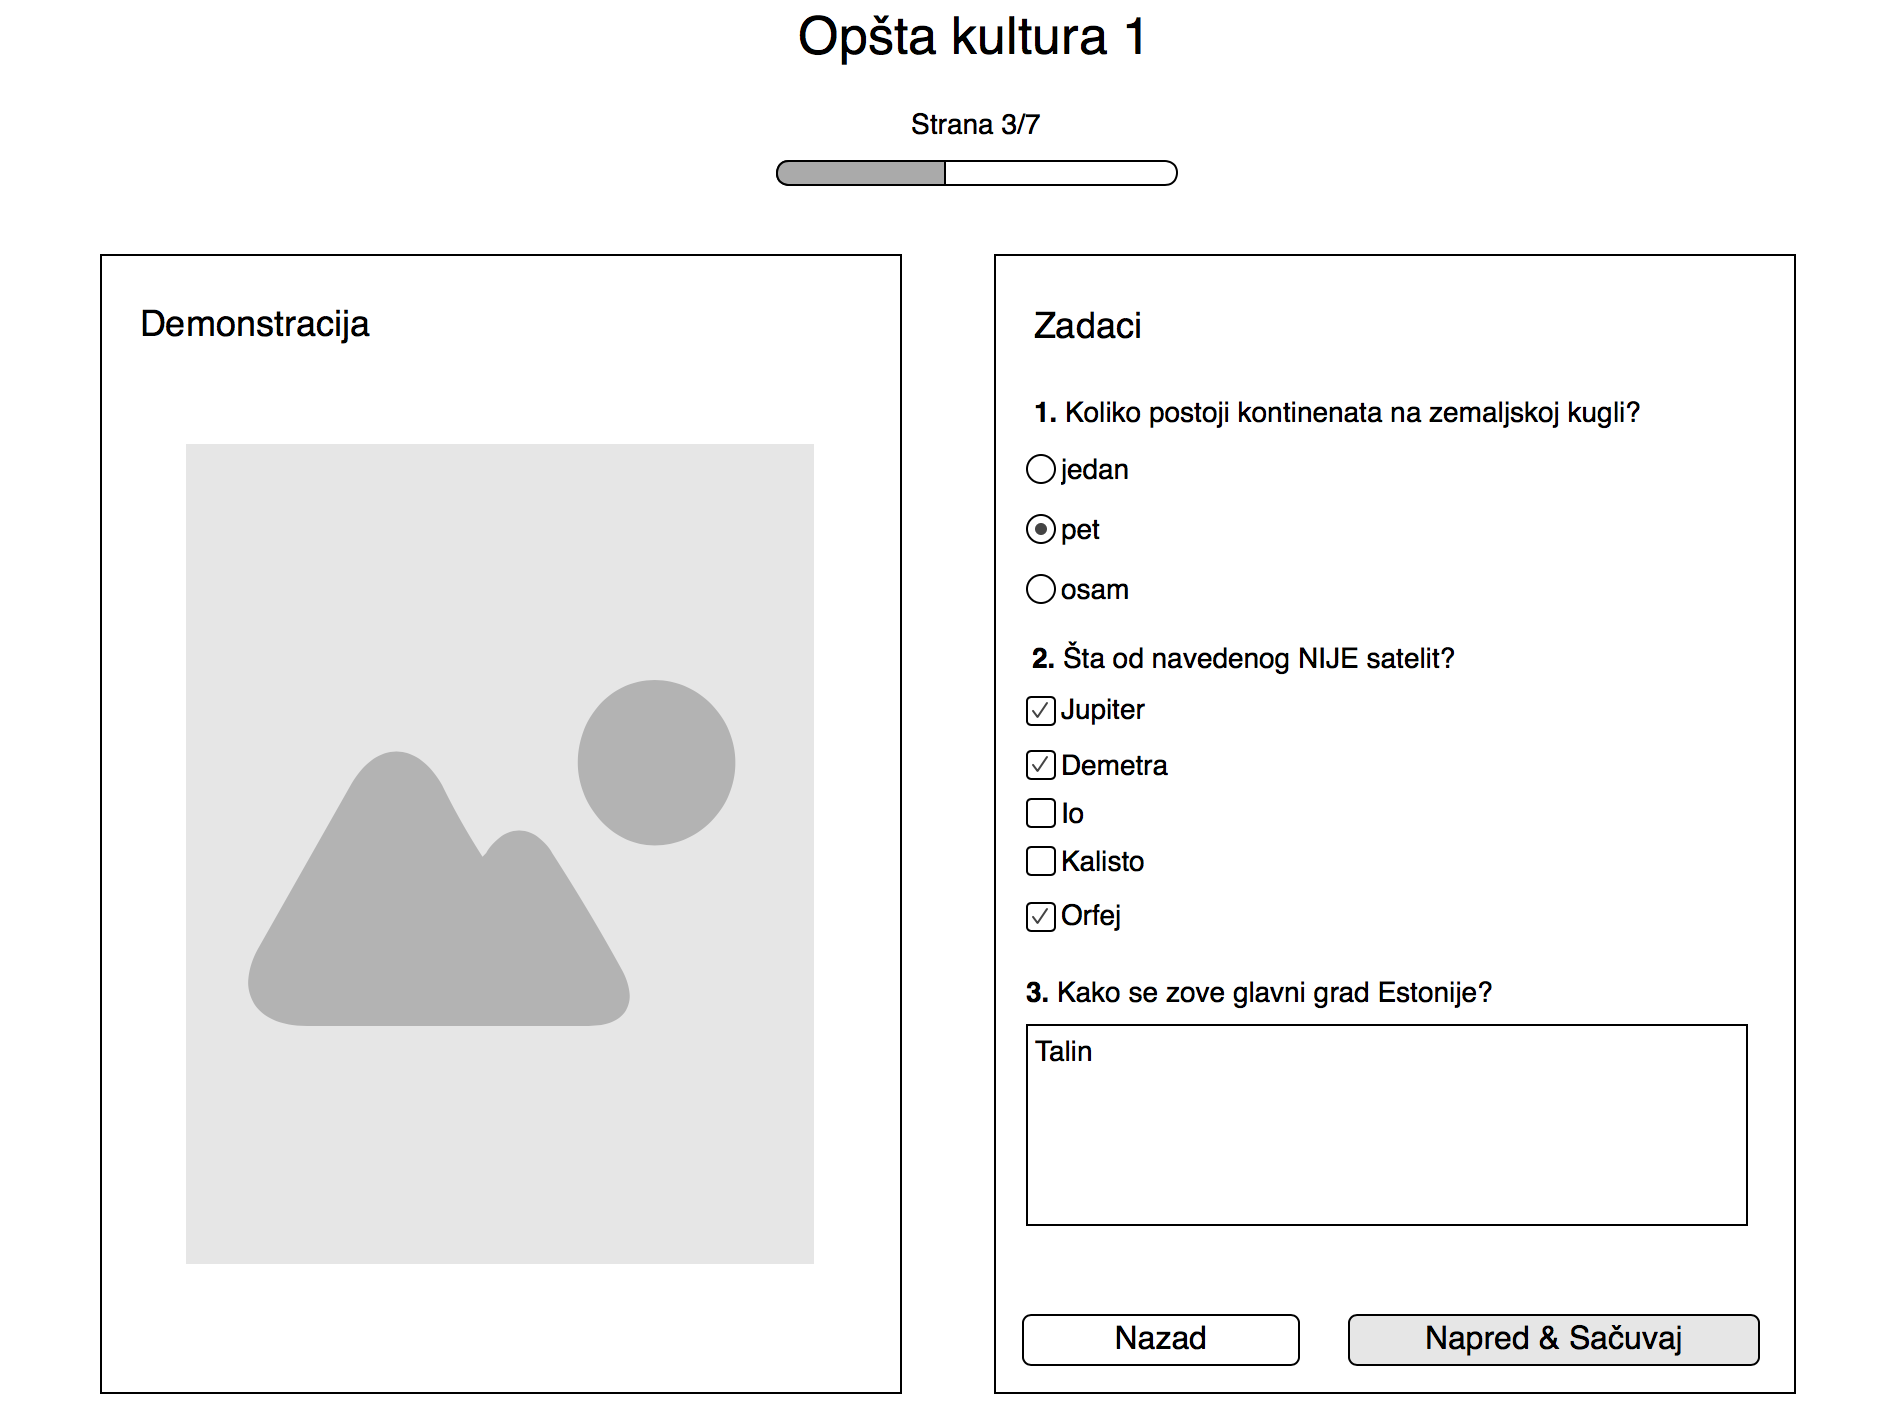
\includegraphics[width=\textwidth]{test-mockup}
\caption{UI \textit{mockup} stranice za polaganje testova}
\label{fig:test-mockup}
\end{figure}

Korisnik može slobodno da se kreće kroz stranice sa pitanjima. Pri tome se čuvaju uneti odgovori na pitanja. Korisnik može preskočiti neka pitanja, ali mu se tada, pre predavanja testa, prikazuje upozorenje da na neka pitanja nije dat odgovor.

Nakon što korisnik odgovori na sva pitanja sa testa, na poslednjoj stranici treba da se pojavi dugme za predavanje testa. Kada korisnik klikne na ovo dugme, test treba da bude automatski ocenjen i trajno unet u bazu. Korisnika tada treba vratiti na stranicu za pregled testova. Time je proces polaganja testa završen.

Ukoliko korisnik u bilo kom trenutku prekine polaganje testa, potrebno je omogućiti nastavljanje polaganja prilikom sledećeg logovanja korisnika. Naravno, treba restaurirati dotadašnji progres polaganja testa.

\subsubsection{Administratorski interfejs}
Za razliku od običnih korisnika, nakon što se administrator uloguje treba prikazati pregled ocenjenih testova studenata. Za svaki odrađeni test treba prikazati naziv testa, ime studenta, datum polaganja i uspešnost. Radi lakšeg prikazivanja rezultata, treba omogućiti sortiranje rezultata po svim kolonama, kao i filtriranje po email nalogu studenta.

% TODO

Administrator treba da ima mogućnost da pregleda svaku instancu završenog testa, tako što mu se prikaže isti interfejs kao za polaganje testa, ali bez mogućnosti menjanja odgovora. Međutim, administrator mora imati mogućnost promene automatske ocene tačnosti odgovora, tj. za svako pitanje administrator može pregaziti automatsku odluku sistema i oceniti odgovor kao tačan, tj. netačan. Ovo je izuzetno bitno za pitanja sa odgovorom u slobodnom stilu.

\subsection{Druga grupa zahteva}
Druga grupa zahteva je vezana za oblast formalne logike, i odnosi se na unos, transformaciju i prikazivanje logičkih izraza.

Za potrebe demonstracije određenih algoritama, kao i za potrebe unosa odgovora na pitanja iz ove oblasti, neophodno je omogućiti unos stavova predikatske logike. Pod ovim se podrazumevaju \textbf{dobro formirane formule} (\textit{well-formed formulae}, skraćeno \textit{wff}, dalje u tekstu samo formule). Formule se sastoje od sledećih elemenata:
\begin{itemize}
\item \textbf{logičkih promenljivih}, koje se obeležavaju malim slovima abecede, na primer $x$ ili $var$,
\item \textbf{predikata ili funkcija}, koji se navode kao reči abecede sa velikim početnim slovom, praćene proizvoljnim brojem logičkih promenljivih, i/ili drugih predikata ili funkcija kao argumentima, npr. $\mathit{Na}(x, y)$, $\mathit{MANJE}(a, b)$ ili $\mathit{PlusJedan}(var)$,
\item \textbf{logičkih operatora}, poimence:
\begin{itemize}
\item binarnog operatora \emph{konjukcije} $\land$,
\item binarnog operatora \emph{disjunkcije} $\lor$,
\item binarnog operatora \emph{implikacije} $\implies$,
\item unarnog operatora \emph{negacije} $\neg$,
\end{itemize}
\item \textbf{logičkih kvantifikatora}, tačnije:
\begin{itemize}
\item \emph{univerzalnog} kvantifikatora $\forall$, i
\item \emph{egzistencijalnog} kvantifikatora $\exists$
\end{itemize}
\end{itemize}
I pored bogatog skupa logičkih simbola, unos formula mora biti moguć preko standardnih znakova koji se unose preko tastature, ili preko ekrana mobilnog uređaja. Osim toga, neophodno je obezbediti i proveru da li je neki arbitraran unos zaista formula. Ova provera bi se idealno mogla izvršavati uporedo sa unosom, nakon svakog unešenog karaktera.

Nezavisno od načina unosa formula, treba implementirati i renderovanje formula, sa akcentom na čitljivosti. U idealnom slučaju, formule treba prikazati u \LaTeX \space \textit{typesetting} formatu.

Kada se govori o transformaciji formula, misli se na svođenje na \textbf{konjuktivnu normalnu formu} (\textit{conjuctive normal form}, skraćeno KNF). Pre definisanja konjuktivne normalne forme, zgodno je uvesti par definicija:
\begin{itemize}
\item \textbf{Atom} je najprostija dobro formirana formula koja se sastoji od logičke varijable ili predikata.
\item \textbf{Literal} je atom ili njegova negacija.
\item \textbf{Klauzula} je skup literala međusobno povezanih disjunkcijama.
\end{itemize}
Sada se konjuktivna normalna forma može definisati kao \emph{konjukcija klauzula}. Iz ovoga sledi da se u KN formi ne pojavljuju kvantifikatori niti operator implikacije, i da je logički operator negacije u KN formi spušten do atomskog nivoa. Značaj KN forme je u tome što je veoma pogodna za korišćenje od strane sistema za automatsko rezonovanje (zaključivanje).

Algoritam transformacije formule u KNF sastoji se od sledećih koraka:
\begin{enumerate}
\item Eliminisanje implikacija
$$ x \implies y \equiv \neg x \lor y $$
\item Primena DeMorgan-ovih zakona i spuštanje negacija do atomskog nivoa
\begin{align*}
\neg(x \land y) &\equiv \neg x \lor \neg y \\
\neg(x \lor y) &\equiv \neg x \land \neg y \\
\neg (\neg x) &\equiv x \\
\neg \forall x \, (P(x)) &\equiv \exists x \, (\neg P(x)) \\
\neg \exists x \, (P(x)) &\equiv \forall x \, (\neg P(x))
\end{align*}
\item Zamena egzistencijalnih kvantifikatora arbitrarnim funkcijama. čiji su argumenti sve promenljive vezane univerzalnim kvantifikatorom na tom mestu u formuli
$$ \forall x \; \exists y \, (P(x, y)) \to \forall x \, (P(x, \Phi(y))) $$
\item Preimenovanje varijabli tako da svakom kvantifikatoru odgovara unikatna promenljiva, na primer:
$$ \forall x \, (P(x)) \land \forall x \, (Q(x)) \to
\forall x \, (P(x)) \land \forall y \, (Q(y)) $$
\item Premeštanje univerzalnih kvantifikatora na početak formule, bez promene redosleda, na prethodnom primeru:
$$ \forall x\, (P(x)) \land \forall y \, (Q(y)) \to
\forall x \; \forall y \, (P(x) \land Q(y)) $$
\item Spuštanje disjunkcija do atomskog nivoa (osobina asocijativnosti)
$$ (x \land y) \lor z \equiv (x \lor z) \land (y \lor z) $$
\item Eliminacija konjukcija razdvajanjem operanada na posebne formule
\begin{align*}
\forall x \; \forall y \; \forall z \, ((x \lor y) \land (y \lor a) \land (z \lor a)) \to \; &\forall x \; \forall y \, (x \lor y) \\
&\forall y \, (y \lor a) \\
&\forall z \, (z \lor a)
\end{align*}
\item Preimenovanje varijabli tako da ne postoje formule sa istim univerzalnim kvantifikatorima, na prethodnom primeru:
\begin{align*}
&\forall x \; \forall y \, (x \lor y) \\
&\forall w \, (w \lor a) \\
&\forall z \, (z \lor a)
\end{align*}
\item Uklanjanje kvantifikatora, na prethodnom primeru:
\begin{align*}
& x \lor y \\
& w \lor a \\
& z \lor a
\end{align*}
\end{enumerate}
Kao deo zahteva druge grupe, neophodno je implementirati automatsku konverziju unesene formule u KNF, sa mogućnošću prikaza rada algoritma po koracima.

% dodati algoritme rezonovanja

\section{Opis korišćenih tehnologija}
\subsection{Izbor jezika}
Online platforma poput izrađene web aplikacije se može realizovati u gotovo svim višim programskim jezicima današnjice. Prednost svakako imaju jezici koji:
\begin{itemize}
\renewcommand\labelitemi{--}
\item su na dovoljno visokom nivou apstrakcije - na primer, podrška za \textit{garbage collection} je obavezna,
\item koji se mogu izvršavati na velikom broju platformi uz minimalne izmene izvornog koda - pre svega, interpreterski jezici i jezici koji se izvršavaju na virtuelnim mašinama, tj. prevode se u bajtkod,
\item dolaze sa kvalitetnom i robusnom standardnom bibliotekom, i za koje postoji veliki broj dostupnih \textit{3rd party} biblioteka, i
\item imaju detaljnu i preglednu dokumentaciju i podršku online zajednice.
\end{itemize}
Sa ovim ne pretarano striktnim ograničenjima na umu, prirodno se nameće veliki broj popularnih jezika: Java, C\#, Python, Go, Rust itd.

Međutim, kako autor tokom dužine studija nije imao priliku da izučava još neku paradigmu osim objektno-orijentisanog programiranja, a vođen idejom da jedan alat nikako ne može da bude pravo rešenje za sve probleme, odluka je pala na \textbf{Clojure}. Clojure je moderni dijalekat LISP-a, i samim tim je funkcionalan jezik. Izvorni kod Clojure programa se prevodi na Java bajtkod, koji se izvršava na Java virtuelnoj mašini\footnote{Osim Java bajtkoda, Clojure kod je moguće pokretati i na \textit{Common Language Runtime} mašini i JavaScript mašini.}. Zbog toga Clojure, pored već bogatog ekosistema raznoraznih biblioteka, ima pristup svim bibliotekama pisanim u Javi. Takođe, Clojure ima veoma aktivnu zajednicu, kao i veliki broj knjiga\cite{Emerick:2012:CP}\cite{Higginbotham:2015:CBT}, priručnika, tutorijala i resursa za učenje.

Jedna prednost Clojure-a nad Javom, koju će autor vremenom naučiti da veoma ceni, jeste postojanje \textbf{REPL} (\textit{read-eval-print-loop}) funkcionalnosti. Radi se o interaktivnoj konzoli u kojoj je moguće unositi i evaluirati delove Clojure koda, veoma slično Python interpreteru. Uz činjenicu da su većina Clojure funkcija \textit{pure}\footnote{Čiste funkcije uvek vraćaju isti rezultat za iste argumente, i nemaju bočne efekte.}, REPL omogućava unikatan način razvijanja aplikacije, gde je funkcija osnovna celina razvoja i testiranja.

Izrađena web aplikacija se sastoji od dva snažno spregnuta dela: \emph{frontend} sistema i \emph{backend} sistema. Kao što im ime kaže, frontend deo je zadužen za prezentacioni sloj i obradu unosa, dok je backend sistem zadužen za perzistenciju i serviranje sadržaja, i veći deo poslovne logike.

\subsection{Backend tehnologije}

\paragraph{HTTP server}
\emph{Ring}\cite{ring} je apstrakcija HTTP servera koja preko veoma jednostavnog API-ja\footnote{\url{https://github.com/ring-clojure/ring/blob/master/SPEC}} omogućava korisniku da se fokusira na implementaciju hendlera (tj. poslovne logike), bez ulaženja u detalje HTTP protokola. API definiše HTTP zahtev i HTTP odgovor kao dve obične Clojure mape, a hendlere kao funkcije koje imaju jedan argument (mapu zahteva) i vraćaju odgovor kao mapu. Zbog toga što Ring predstavlja apstrakciju HTTP servera, Ring web aplikacije mogu da se distribuiraju kao WAR aplikacije i pokreću unutar standardnih kontejnera za web aplikacije (npr. Tomcat), ili da se pokrenu same pomoću \textit{embedded} Jetty web servera, što je za potrebe ove web aplikacije više nego dovoljno.

\paragraph{Rutiranje}
Ring API je previše jednostavan za neke iole ozbiljnije zahteve, te je zbog toga nastao \emph{Compojure}\cite{compojure}, koji je \textit{routing} biblioteka za Clojure. Jednostavno rečeno, ova biblioteka prosleđuje određene HTTP zahteve (\texttt{GET}, \texttt{POST} itd.) za URI putanjama (tj. resursima) hendlerima koji ih obrađuju. Tako je, na primer, moguće napraviti hendler koji vraća početnu stranicu ukoliko se ka serveru uputi HTTP \texttt{GET} zahtev za \texttt{/index.html} resursom. Međutim, \texttt{POST} zahtevi ka istom resursu će biti odbijeni sa statusom \texttt{403 Forbidden}. Ovaj postupak uparivanja resursa i hendlera se naziva rutiranje.

\paragraph{Šabloni} Server generiše HTML stranice na upit pomoću mašine za šablone (\textit{template engine}). U ovu svrhu je korišćena jednostavna Clojure biblioteka pod nazivom \emph{Hiccup}\footnote{\url{https://github.com/weavejester/hiccup}}. Jedinstvena je po tome što nema statičke šablonske fajlove, već DOM stablo HTML dokumenta predstavlja preko Clojure struktura podataka, na primer \texttt{[:div \string{:id "header"\string} [:h1 "Header"]]}.

\paragraph{Perzistencija}
Kako korisnički zahtevi nameću, svi podaci o testovima, polaganju testova, registrovanim korisnicima itd. moraju se trajno negde smestiti, tj. moraju biti perzistentni. Standardna rešenja za perzistenciju predstavljaju relacione baze podataka. Autor se odlučio za \emph{PostgreSQL}\cite{postgres}, pre svega zbog postojećeg iskustva sa ovim RDBM sistemom.

\paragraph{Objektno-relaciono mapiranje}
ORM je strategija povezivanja stanja objekata u memoriji sa stanjem odgovarajućih objekata u relacionoj bazi. Iako su Clojure programima dostupne Java biblioteke koje predstavljaju industrijski standard (na primer, Hibernate), autor se odlučio za laganiju varijantu - za pristup bazi se koristi JDBC drajver za Postgres i mala Clojure biblioteka zvana \emph{YeSQL}\footnote{\url{https://github.com/krisajenkins/yesql}}. Ova biblioteka čita SQL skripte sa upitima, i za svaki upit pravi Clojure funkciju preko kojih je moguće proslediti imenovane parametre u upit, na sličan način na koji se to radi sa \texttt{NamedQuery} objektima u \textit{Java Persistence Language}-u. Nije razmatrana upotreba \textit{connection pooling}-a za konekcije ka bazi. Međutim, ukoliko se ukaže potreba za time, dodavanje takve biblioteke je prosto.

\paragraph{Parsiranje logičkih jednačina} Mesto ručne izrade leksera i parsera za unošenje logičkih jednačina, autor se odlučio da iskoristi sjajnu Clojure biblioteku \emph{Instaparse}\cite{instaparse} za generaciju parsera bezkontekstnih gramatika. Ova biblioteka generiše parser na osnovu specifikacije gramatike u EBNF obliku. Pri tome podržava levu i desnu rekurziju i regularne izraze. Izlaz parsera je stablo parsiranja u obliku standardnog Clojure vektora. Instaparse može da parsira i dvosmislene gramatike, tako što vraća sekvencu svih mogućih stabala parsiranja.

\paragraph{Ostalo} Za logovanje se koriste već dobro poznata rešenja u vidu \emph{Log4j} biblioteke i \emph{SLF4j} fasade. Konfiguracija sistema vrši se preko EDN (\textit{Extensible Data Notation}) datoteka i biblioteke zvane \emph{Immuconf}. EDN je zapravo podskup Clojure jezika, i predstavlja standard za serijalizaciju podataka. \textit{Cheshire} se koristi za konverziju Clojure podataka u JSON format, i obratno. Konačno, \textit{Postal} biblioteka se koristi za slanje email poruka sa lozinkom korisnicima nakon uspešne registracije.

\subsection{Frontend tehnologije}

\emph{AngularJS}\cite{angularjs} je korišćen kao \textit{de facto} standard za frontend JavaScript framework, u kombinaciji sa \emph{Bootstrap}\cite{bootstrap} CSS stilovima. Angular je uglavnom korišćen za validaciju obrazaca i POST zahteve ka serveru u pozadini, dok Bootstrap obezbeđuje podrazumevanu temu ugodnu za oko, ikonice, i fluidan \textit{layout} stranice koji automatski prilagođava stranicu tipu uređaja, bilo da je to desktop ili mobilni internet pregledač. HTML stranice su u skladu sa HTML5 standardom.

% TODO reci da se koristi bootstrap module for angular, da se ne koristi bootstrap JSS ni jquery

Za prikazivanje logičkih jednačina koristi se JS biblioteka \emph{KaTeX}\footnote{\url{https://github.com/Khan/KaTeX}}, koja omogućava efikasno renderovanje jednačina u \LaTeX formatu.

\subsection{Alati za kompajliranje, pakovanje i distribuciju aplikacije}

% TODO Leiningen

\chapter{Opis rada sistema}\label{sistem}
U ovom poglavlju se detaljno izlaže opis rada sistema iz dve perspektive: perspektive studenta - korisnika sistema, i perspektive profesora - administratora sistema.

\section{Opis rada sistema iz perspektive studenta}
\subsection{Logovanje na sistem i registracija}
Prva stranica koja se prikazuje kada korisnik uputi pretraživač na adresu servisa jeste login stranica, prikazana na slici \ref{fig:login}. Na ovoj stranici korisnik unosi svoju email adresu i lozinku i nakon toga se loguje na sistem pritiskom na dugme \textbf{Prijava}. Prihvataju se samo email adrese koje se završavaju sa \texttt{@etf.rs}. Email adresa se dinamički proverava dok je korisnik unosi, i to tako da je dugme za prijavu onemogućeno dok se ne unese korektna adresa.
\begin{figure}[p]
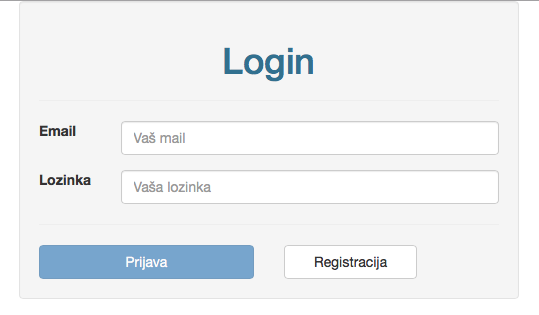
\includegraphics[width=0.5\textwidth]{login}
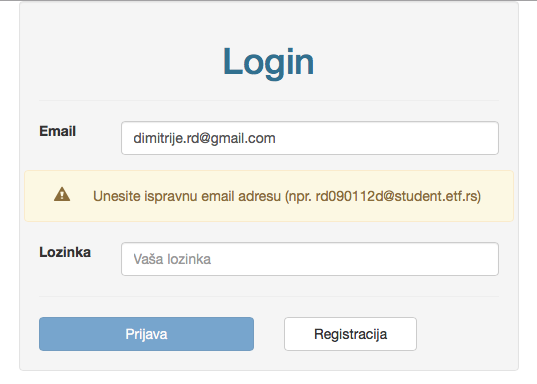
\includegraphics[width=0.5\textwidth]{login-wrongemail}
\caption{Levo: inicijalni izgled login stranice, desno: login stranica tokom unosa email adrese}
\label{fig:login}
\end{figure}
Pokušaj prijave korisnika koji nije registrovan, ili koji se ulogovao sa pogrešnom lozinkom se prikazuju kao greška (slika \ref{fig:login-error}).
\begin{figure}[p]
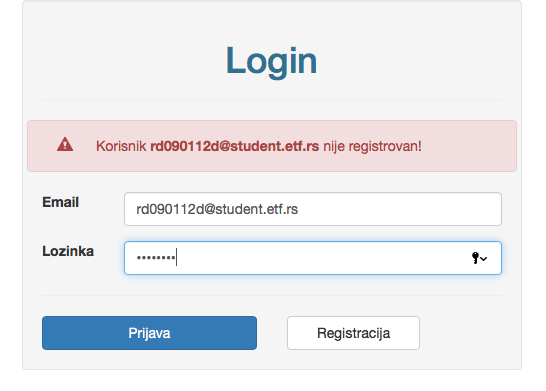
\includegraphics[width=0.5\textwidth]{login-error-unknown}
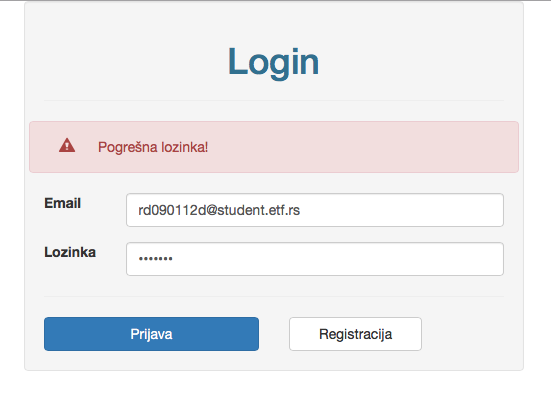
\includegraphics[width=0.5\textwidth]{login-error-password}
\caption{Login stranica nakon što neregistrovani korisnik pokuša da se uloguje (levo), ili ukoliko korisnik unese pogrešnu lozinku (desno)}
\label{fig:login-error}
\end{figure}

Novi korisnici mogu da se registruju pritiskom na dugme \textbf{Registracija}. Ta akcija ih vodi na stranicu za registrovanje novih korisnika (slika \ref{fig:register}), koja od korisnika traži da unese email adresu (ista ograničenja vezana za email adresu se primenjuju i ovde). Pokušaj postojećeg korisnika da se ponovo registruje rezultuje greškom. Nakon što unese email, pritiskom na dugme \textbf{Izvrši} se korisnik registruje na sistem. Nakon uspešne registracije korisniku se prikazuje stranica sa slike \ref{fig:register-success}. Tom prilikom se na unetu email adresu automatski šalje email sa nasumično generisanom lozinkom za tog korisnika. Sa ovom lozinkom korisnik sada može da se uloguje na sistem preko stranice za logovanje.
\begin{figure}[p]
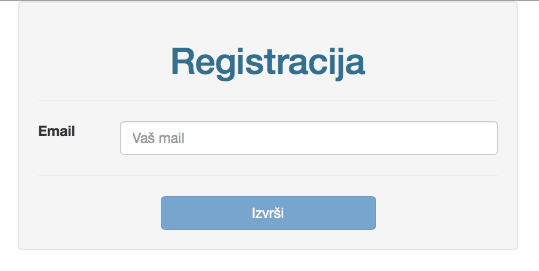
\includegraphics[width=0.5\textwidth]{register}
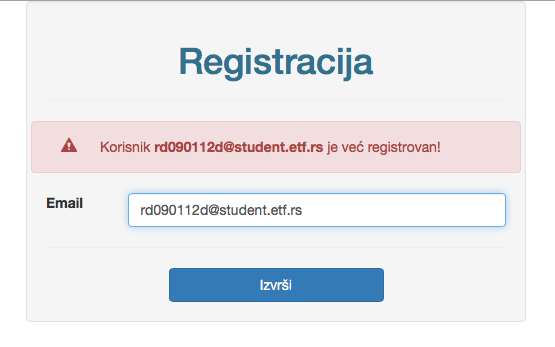
\includegraphics[width=0.5\textwidth]{register-error}
\caption{\textit{Levo}: inicijalni izgled stranice za registrovanje, \textit{desno}: stranica za registracije nakon što već registrovani korisnik pokuša da se registruje}
\label{fig:register}
\end{figure}
\begin{figure}[h]
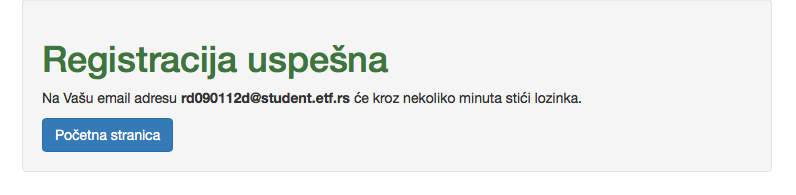
\includegraphics[width=\textwidth]{register-success}
\caption{Izgled stranice za registraciju nakon uspešne registracije}
\label{fig:register-success}
\end{figure}

\subsection{Stranica sa pregledom testova}
Nakon uspešne prijave na sistem, korisniku se prikazuje stranica sa pregledom svih testova trenutno u sistemu. Ova stranica se prikazuje i kao početna stranica ukoliko je korisnik već ulogovan na sistem, a pregledač usmeri na \textit{root} URL servisa. Testovi su grupisani po kategorijama, i prikazani unutar tabele u svakoj kategoriji. Za svaki test se prikazuje ime testa, broj stranica sa pitanjima, i ukupan broj pitanja. Testovi koji se prikazuju na ovoj stranici se dele na:
\begin{itemize}
\renewcommand\labelitemi{--}
\item \textbf{Završene testove}, tj. testove koje je korisnik predao. Za ove testove se dodatno prikazuju datum i vreme kada je test započet, datum i vreme kada je test završen, procenat od ukupnog broja pitanja na koja je student dao odgovor, tj. progres, i najzad ocena, u vidu procenta tačnih odgovora u odnosu na ukupan broj pitanja. Boja pozadine ovih unosa je zelena.
\item \textbf{Testove u toku}, tj. testove koje je korisnik započeo, ali nije završio. Za ove testove se dodatno prikazuju datum i vreme kada je test započet, progres, i link ka stranici sa testom. Boja pozadine ovih unosa je žuta.
\item \textbf{Nezapočete testove}, tj. testove koje korisnik nikada nije polagao. Za ove testove se dodatno prikazuje link ka stranici sa testom. Boja pozadine ovih unosa je bela.
\end{itemize}

\chapter{Realizacija sistema}\label{realizacija}
Realizacija
\chapter{Zaključak}\label{zakljucak}
Zaključak
\renewcommand\bibname{Reference}
\printbibliography
\end{document}